\documentclass{endm}
\usepackage{endmmacro}
\usepackage{graphicx}
\usepackage{indentfirst}
\usepackage{lscape}
\usepackage{CJK}
\usepackage{epsfig}

\usepackage{amsmath}
\usepackage{subfigure}
\usepackage{hyperref}
\usepackage{multirow}
% The following is enclosed to allow easy detection of differences in
% ascii coding.
% Upper-case    A B C D E F G H I J K L M N O P Q R S T U V W X Y Z
% Lower-case    a b c d e f g h i j k l m n o p q r s t u v w x y z
% Digits        0 1 2 3 4 5 6 7 8 9
% Exclamation   !           Double quote "          Hash (number) #
% Dollar        $           Percent      %          Ampersand     &
% Acute accent  '           Left paren   (          Right paren   )
% Asterisk      *           Plus         +          Comma         ,
% Minus         -           Point        .          Solidus       /
% Colon         :           Semicolon  7  ;          Less than     <
% Equals        =           Greater than >          Question mark ?
% At            @           Left bracket [          Backslash     \
% Right bracket ]           Circumflex   ^          Underscore    _
% Grave accent  `           Left brace   {          Vertical bar  |
% Right brace   }           Tilde        ~

\newcommand{\Nat}{{\mathbb N}}
\newcommand{\Real}{{\mathbb R}}
\def\lastname{Ye}

\begin{document}

\begin{CJK}{UTF8}{song}
% DO NOT REMOVE: Creates space for Elsevier logo, ScienceDirect logo
% and ENDM logo
\begin{verbatim}\end{verbatim}\vspace{2.5cm}


\begin{frontmatter}
% \title{A Graph based Approach to Mine Multilingual Word Associations from Wikipedia}
\title{Segments: A Foreign Name Search Algorithm}


\author{Jason Soo \thanksref{myemail}}
\address{School of Computer Science\\ Georgetown University\\ Washington, DC, USA}


\author{Ophir Frieder \thanksref{ofemail}}
\address{School of Computer Science\\ Georgetown University\\ Washington, DC, USA}

\thanks[myemail]{Email:
   \href{mailto:soo@ir.cs.georgetown.edu} {\texttt{\normalshape
   soo@ir.cs.georgetown.edu}}} 
\thanks[ofemail]{Email:
   \href{mailto:ophir@ir.cs.georgetown.edu} {\texttt{\normalshape
   ophir@ir.cs.georgetown.edu}}} 

\newpage
\begin{abstract}
	We address foreign name search in a highly diverse user community.  User sophistication ranges from highly experienced archivists to apprehensive users who shy away from technology; apprehensive users dominate system use.  Thus, all system interfaces must assume minimal dependency on the user. 

	Our foreign names search approach, called S\textsc{egments}, is language independent; thus, there is no need to determine the language of origin from the diverse candidate set of thirteen languages.  We compare S\textsc{egments} against traditional n-gram and Soundex based solutions.  Actual and synthetic queries are used to search a names data set resident in the United States Holocaust Memorial Museum.  We also search a subset of the 1990 United States Census Bureau Surnames data set to evaluate the performance of S\textsc{egments} on a predominately language specific (English) collection.  Our results demonstrate statistically significant performance gains over both traditional approaches.  The described approach supports search efforts at the United States Holocaust Memorial Museum.
\end{abstract}
\begin{keyword}
Foreign Name Search, Substring Matching
\end{keyword}

\end{frontmatter}

\section{Introduction}\label{s:introduce}
Name identification significantly impacts accuracy in the general search case; however, in historical document search, their identification is paramount.  Complicating name search is the variance of accepted spellings for the same sounding name, for example Laurence and Lawrence.  To circumvent spelling issues, phonetic search techniques are often used \cite{zobel:phonetic}.  Common phonetic techniques are based on Soundex; JewishGen \cite{jewishgen.org} uses the Daitch-Mokotoff (D-M) Soundex variant \cite{mokotoff:soundexing}, a de facto standard by Jewish genealogical organizations.  

A difficulty with using phonetic search stems from the reliance on the user to formulate an approximate sound, and hence spelling, of the foreign name.  For example, to an English speaker, \emph{``Roz'ishts' \'avarati''} or \emph{``Rozhyshche''} is likely to be difficult to pronounce.  Furthermore, in searching name indices from historical documents, particularly for personal-data related applications such as JewishGen genealogy \cite{jewishgen.org} or Yizkor Books \cite{amir:from}, often the user knows that the name of interest has an ``esto'' in it (from a name like: Nov\'e Mesto nad V\'ahom) but is uncertain about the remainder of the name or even the language that the name is in.  This occurs fairly often since a variety of communities existed in each location.  For example, for the German speaking community in Czechoslovakia during the 1930's, ``Nov\'e Mesto nad V\'ahom'' was called ``Neustadt an der Waag'', and ``Bratislava'' was called ``Pressburg'' by German speakers and ``Pozsony'' by Hungarian speakers.  In the hope that some fragment of the name will match, which obviously is not always the case, n-gram based solutions \cite{manning:introduction} are deployed.  

Earlier efforts \cite{aljlayl:on,aqeel:on,guy:the} have demonstrated that efficient simple rules can outperform many traditional approaches. Our language-independent name search approach, called S\textsc{egments}, follows this trend.  That is, we search a collection of foreign names by segmenting the input string according to a set of simple rules. The search results obtained using the individual segments are merged, and a confidence for the merged list is derived.  If the confidence is insufficient, namely below a predefined threshold, we invoke an n-gram search.  

Extracting from a database of names derived from various documents and texts resident at and/or accessed by the United States Holocaust Memorial Museum, we favorably compare the search accuracy of S\textsc{egments} against traditional n-gram and D-M Soundex based solutions. Actual user queries as well as synthetic queries generated using single and multiple character addition, deletion, replacement, and inversion are used in our evaluation.  We also show favorable results using a subset of the 1990 United States Census Bureau collection of surnames \cite{us_census_bureau}.  A subset rather than the entire collection was chosen so as to mirror the size of the United States Holocaust Memorial Museum data set used.  S\textsc{egments} is used in support of search efforts for the United States Holocaust Memorial Museum.  

\section{Yizkor Book Metadata Search: A S\textsc{EGMENTS} Application} % (fold)
\label{sec:yizkor_book_metadata_search}

The Yizkor Book Metadata Search project, an effort led by the Archives Section of the United States Holocaust Memorial Museum, aims to create an online metadata global directory of Yizkor Books.  Briefly, Yizkor Books memorialize life before, during, and after the Holocaust describing everyday events including births, marriages, and deaths.  Many texts were written by survivors or their relatives or friends as a tribute to those who perished.  Most texts are written using multiple languages.  Thirteen languages are used: Czech, Dutch, English, French, German, Hebrew, Hungarian, Lithuanian, Polish, Romanian, Serbo-Croatian, Spanish, and Yiddish.  Given the diversity of languages, only a language independent approach is viable. 

% Old Yizkor figure placeholder


Yizkor books are scattered globally, but currently, a global directory of these books is unavailable.  Some Yizkor Book repositories go as far as to provide download-ready, scanned copies of the books, for example those residing within the New York City Public Library \cite{nypl.org}; however, locating some of these digital repositories, particularly the lesser ones, is accomplished mainly by word of mouth.   

The preliminary architecture of Yizkor Books metadata search system was initially described in \cite{soo:yizkor}.  Here, in Figure~\ref{fig:yizkor_overview}, we illustrate the currently deployed architecture.  As shown, metadata are generated internally by USHMM staff or fellows, generated externally by a diversity of users including historians, genealogists, librarians, etc. or are downloaded directly from Yizkor Book repositories and sent via the Internet to the metadata search engine.  Once collected, they are organized, temporarily housed in a verification repository (not illustrated), and eventually stored in the Yizkor Books metadata repository.  To guarantee correctness, a temporary verification repository is used as an intermediary.  That is, all metadata are inspected and verified for accuracy by authorized personnel prior to insertion into the metadata repository.  Thus, there are always ``humans in the loop''.

\begin{figure}
\centering
%\vspace{0.5cm}
\epsfig{file=yizkor_flow.eps,width=3in}
%\includegraphics[width=3in]{yizkor_flow.png}
\caption{Yizkor Overview}
\label{fig:yizkor_overview}
\end{figure}

\begin{figure}
\centering
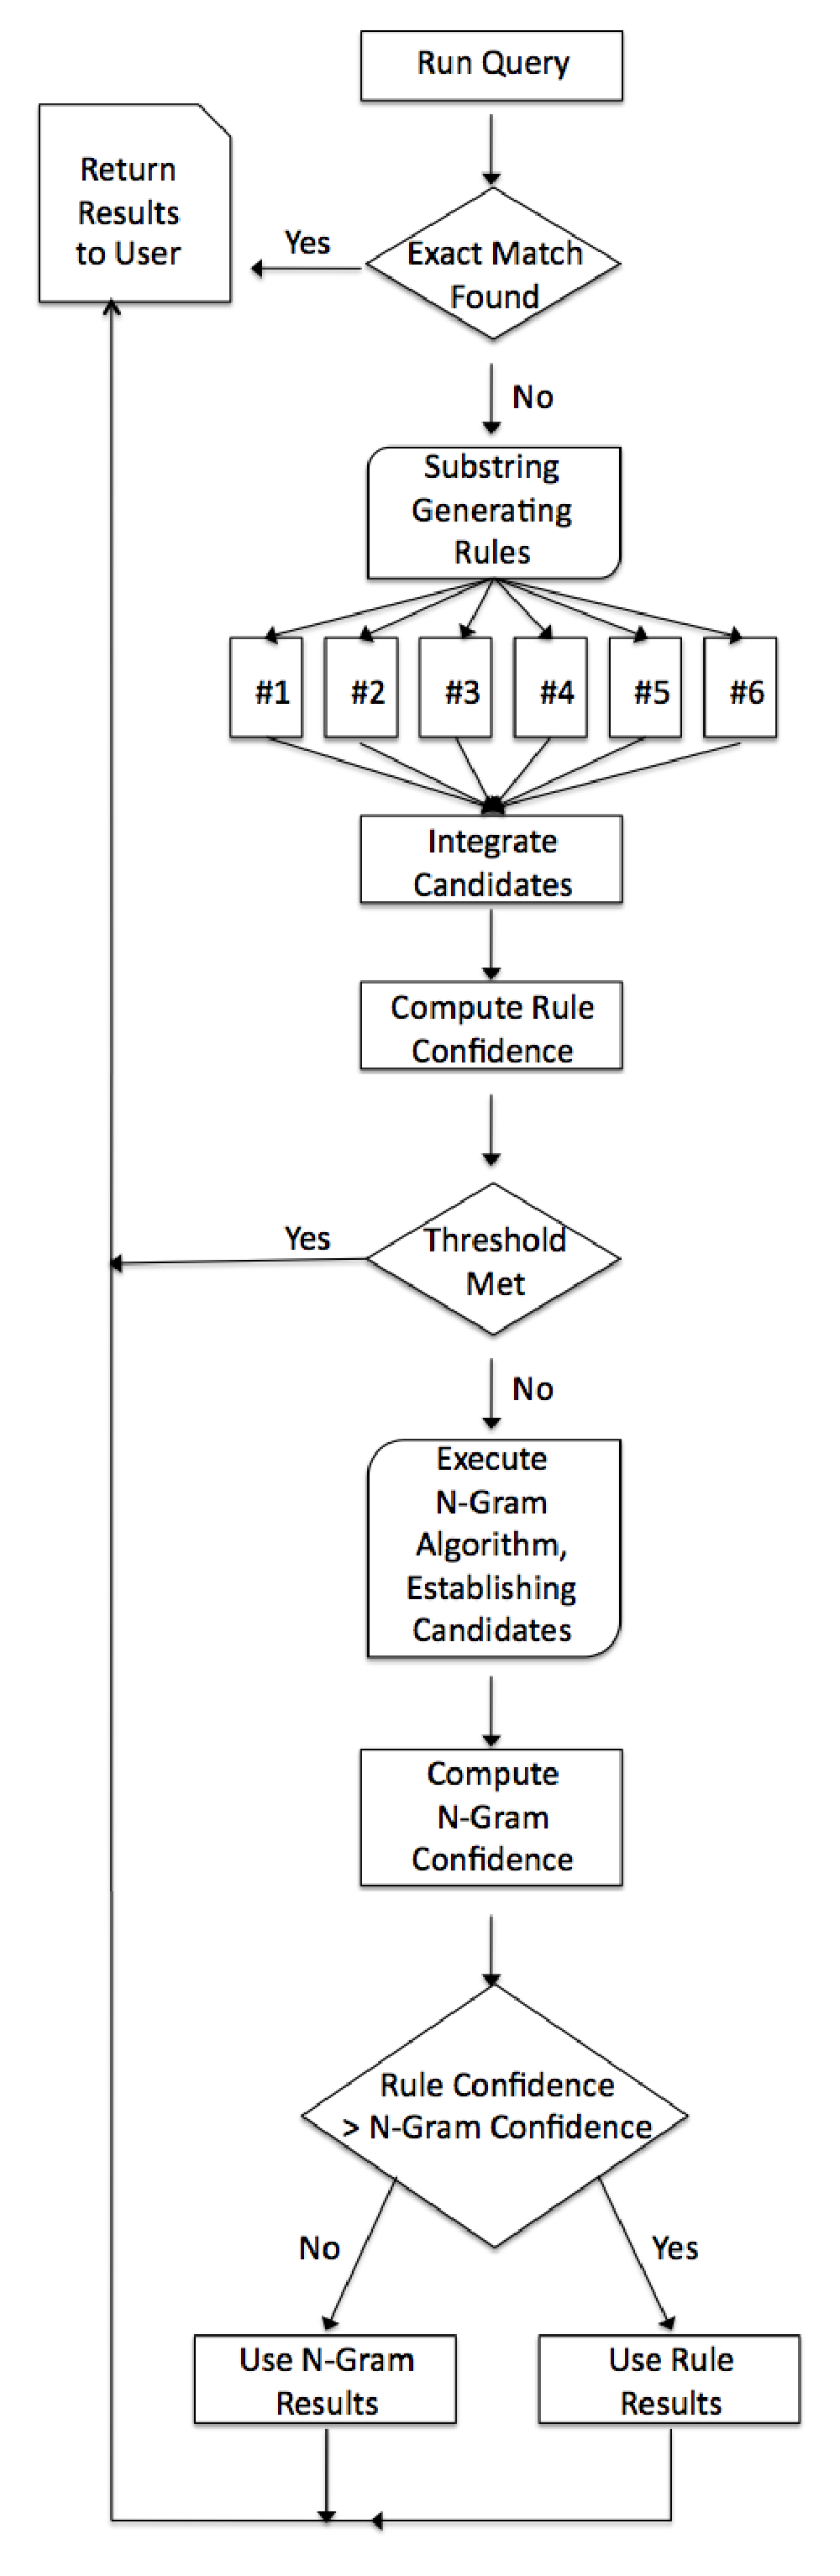
\epsfig{file=segments_flow.eps,height=8.1in,width=3in}
%\includegraphics[height=8.35in,width=3in]{}
\caption{Query Processing Overview}
\label{fig:segments_overview}
\end{figure}


User queries from a diverse audience are issued and sent likewise via the Internet to the metadata search engine.  S\textsc{egments} is the foreign name search component within the search engine.  The queries are translated to the appropriate internal format, issued against the repository, and corresponding metadata are returned.  The candidate results are then returned to the user.
% section yizkor_book_metadata_search_systems (end)


\section{Algorithm} % (fold)
\label{sec:algorithm}
Our S\textsc{egments} approach operates as shown in Figure~\ref{fig:segments_overview}.  Initially the user generated query is issued against the name index derived from the collection.  No attempt is made to identify the language.  If an exact match is found, then the matching name or names and their corresponding information are returned with a confidence of 1.  Otherwise, multiple substrings are derived applying simple substring generating rules.  The collection is then searched using these derived substrings.  Many substring generating rule variations were studied; the deployed system uses:

\begin{itemize}
	\item Rule 1:  Replace first and last characters by a wild card, in succession;
	\item Rule 2:  Replace middle n-characters by a wild card, in succession;
	\item Rule 3:  Replace first half of the string by a wild card;
	\item Rule 4:  Replace second half of the string by a wild card;
	\item Rule 5:  Retain only first and last characters and insert a wild card;
	\item Rule 6:  Retain only first and last two characters and insert a wild card;
\end{itemize}

Generating Rules 1 and 2 are recursive, and thus, can generate a large number of potential substrings.  For Rule 2, typically n=1; however, for substantially long names (greater than 20 characters), n=2.   Note that all names are stored in lower-case.  To limit the search time, only up to three substrings are generated per rule.  Thus, in the deployed implementation, at most ten substrings are generated: three per each of the first two rules and one each for the remaining rules.  In future work, we will study in greater detail which S\textsc{egment} rule is most affective and assign.  The derived substrings for the search term ``Rozhyshche'' are illustrated in Table~\ref{tab:example_phases}.


\emph{Example table omitted for now...}

%\begin{table}
%	\centering
%	\caption{Actual Query Performance Evaluation}
%	\begin{tabular}{|c|c|c|c|c|}
%	\hline
%	\textbf{Rule \#} & \multicolumn{3}{c|}{Search Candidates}\\
%	\hline
%	1 & \%ozhyshch\% & \%zhyshc\% & \%hysh\%\\
%	\hline
%	2 & rozhy\%hche & rozh\%hche & rozh\%che\\
%	\hline
%	3 & \%shche & - & -\\
%	\hline
%	4 & rozhy\% & - & -\\
%	\hline
%	5 & r\%e & - & -\\
%	\hline
%	6 & ro\%he & - & -\\
%	\hline
%	\end{tabular}
%	\label{tab:example_phases}
%\end{table}


For each generated substring, according to its similarity to the desired name, a confidence is determined.  Confidence is defined as the summation of all substring matching algorithms which found (voted for) a candidate word over the total number of casted votes.  The global confidence of the merged result set is computed.  Although multiple generating rules derive some identical candidate strings, this replication was experimentally observed as needed to bolster the confidence.  Clearly, our description of the approach is strictly for clarity of presentation; the actual implementation does not replicate the search, rather candidate weights are adjusted accordingly.  

If the global confidence fails to meet the needed threshold, an n-gram based solution is deployed.  That is, in addition to the segment search already performed, a traditional n-gram search where n=3 is conducted, and a confidence for the n-gram solution is computed.  A comparison of the confidence of S\textsc{egments} and the n-gram solution is made and the option with the higher confidence is selected. Our test data, as well as other related data, are available at http://yizkor.cs.georgetown.edu/collections.
% DOUBLE BLIND
% section algorithm (end)


\section{Soundex} % (fold)
\label{sec:soundex}

To illustrate how S\textsc{egments} avoids problems faced by Soundex and D-M Soundex, a brief overview of these algorithms  is necessary. 
%In our brief review, we use the terms Soundex and D-M Soundex somewhat interchangeably as they use the same basic algorithm with slight encoding variations.


\subsection{Soundex Overview} % (fold)
\label{sub:soundex_overview}

Soundex masks like-sounding characters by replacing them with integer representations, where said integers map to a set of characters.  For example, in Soundex the integer 5 represents either \emph{``m''} or \emph{``n''}.  
%(D-M Soundex, the Eastern European derivative, adjusts the elements of the character sets accordingly.) 
Furthermore, Soundex does not encode the first letter of the given query.  Consider the word ``Slovakia'', which Soundex encodes as ``S412'' \cite{mokotoff:soundexing}.  Details of the Soundex algorithm are omitted since only basic knowledge is required to understand the pitfalls.

% subsection soundex_overview (end)

\subsection{Soundex Pitfalls} % (fold)
\label{sub:soundex_s_pitfalls}


S\textsc{egments} addresses multiple known Soundex pitfalls.  
%Although these issues do not relate directly to D-M Soundex, Soundex has the same basic algorithm as D-M Soundex; they primarily differ in their numerical representation of character groups.  
A subset of these known problems \cite{patman:is}, which S\textsc{egments} resolves are:


\begin{enumerate}
	\item \textbf{\emph{Dependence on initial letter.}}  If the first letter of the user's query is incorrect, Soundex will never find the correct result \cite{patman:is}.  S\textsc{egments} however has 2 rules which will find the correct match.
	\item \textbf{\emph{Noise intolerance.}}  \cite{damerau:a,mitton:spellchecking,pollock:automatic} find that 80\%-95\% of misspellings within large documents are 1) one character insertions 2) one character deletions 3) one character replacements or 4) adjacent character swapping.  Soundex, as demonstrated by \cite{patman:is}, is unable to reliably resolve such noise.  S\textsc{egments} however has demonstrated its tolerance for noise as shown in Tables~\ref{tab:performance_eval} and \ref{tab:us_census_bureau_performance_eval}.
	\item \textbf{\emph{Poor precision.}}  One of the strengths of Soundex is the encoding of words as integers representing character groups.  This representation however leads to ambiguity and ultimately degrades precision.  For example, Soundex encodes the misspelled string ``disapont'' as ``D215''.  A query would then be run for ``D215'' which would return: \textit{disband, disbands, disbanded, disbanding, disbandment, disbandments, dispense, dispenses, dispensed, dispensing, dispenser, dispensers, dispensary, dispensaries, dispensable, dispensation, dispensations, deceiving, deceivingly, despondent, despondency, despondently, disobeying, disappoint, disappoints, disappointed, disappointing, disappointedly, disappointingly, disappointment, disappointments, disavowing} \cite{mitton:spellchecking}.  Should a query be correctly spelled, Soundex will still return several matches for the same reason.  S\textsc{egments} does not suffer from the same ambiguity due to the voting process of the substring matching algorithms used.  Since the above words all have the same encoding, ranking is usually done by frequency \cite{chakkrit:novel}.
\end{enumerate}
% subsection soundex_s_pitfalls (end)

\subsection{D-M Soundex} % (fold)
\label{sub:d_m_soundex}

D-M Soundex, the Eastern European derivative, adjusts the elements of the character sets for language localization.  It also improves upon the Soundex algorithm in the following select ways (localization changes/improvements are omitted)\cite{mokotoff:soundexing}:

\begin{enumerate}
	\item Encoding of the initial letter.  Consider the previous example ``Slovakia'', which Soundex encodes as ``S412''.  In D-M Soundex ``Slovakia'' becomes ``487500''.  Notice the extended length of the D-M Soundex encoding, that is the second improvement.
	\item The first six (rather than four) significant codes are created.  For example, Peters and Peterson have an identical encoding in Soundex (``P362''), but different in D-M Soundex (``739400'', ``739460'').
\end{enumerate}

These changes partially improve some of the downfalls of Soundex (\ref{sub:soundex_s_pitfalls}).  For example, the first pitfall noted, \emph{Dependence on initial letter}, is clearly solved by the first improvement.  The second improvement aids the third pitfall, \emph{Poor precision}, but adds to the time and space complexity.  The \emph{noise intolerance} pitfall however is not addressed, and is the root cause of the majority of misspellings.  In fact, generally if any word contains more than four (Soundex) or six (D-M Soundex) consonants, all characters thereafter are ignored \cite{alexander:beider}. Therefore, neither Soundex or D-M Soundex are viable solutions for users, regardless of their knowledge of a language.

% subsection d_m_soundex (end)

% section soundex (end)


\section{Evaluation} % (fold)
\label{sec:evaluation}
To evaluate our proposed approach, we randomly selected a subset of roughly 1,000 names from the Jewish Census residing at the United States Holocaust Memorial Museum.  Names averaged 8 characters in length, with a median length of 8, a max length of 23, and a standard deviation of 2.8 characters.  Using a set of 250 actual queries, we favorably compared the performance of S\textsc{egments} against the popular D-M Soundex approach and a traditional n-gram solution.

Two metrics were used, namely the percentage of names correctly identified and the average rank of those names found.  A name was defined as found if it ranked in the top 60 entries (first three screens with 20 names listed per screen). Although we evaluated multiple n-values in the n-gram approach, we present results for only n=3, as it consistently supported the highest percentage found.  Average rank rather than MRR is presented as it better illustrates the difference.  Undetected entries are ignored in terms of the average rank computation.  The statistical t-test was used to verify significance.


In Table~\ref{tab:query_performance}, we present our findings using the collected actual 250 queries.  Three measures (percentage found, average rank, and common average rank) for each of three approaches (D-M Soundex, 3-Grams, and S\textsc{egments}), when appropriate, are shown.  The percentage of correctly identified names is presented in the percentage found column.  Since the percentage of correctly identified names is higher when using S\textsc{egments} rather than 3-grams, a common column is presented to provide direct comparison of S\textsc{egments}’ average rank when only considering names also correctly identified by 3-grams.  The percentage of correctly identified names is presented in the percentage found column. Both S\textsc{egments} and 3-Grams statistically significantly (p$<$0.01) outperform D-M Soundex in terms of the percentage of correctly identified names.  S\textsc{egments} likewise statistically significantly (p$<$0.01) outperforms 3-Grams in terms of the percentage of correctly identified names.  


\begin{table}
	\centering
	\caption{U.S. Holocaust Memorial Museum Live Query Performance Evaluation}
	\begin{tabular}{|l|c|c|c|}
		\hline
		 & \textbf{Percentage} & \textbf{Average} & \textbf{Average}\\
		 & \textbf{Found} & \textbf{Rank} & \textbf{Rank}  \\
		 & & & \textbf{(Common)} \\
		\hline
		\textbf{D-M} & 27.56 & 1.03 & N/A \\
		\textbf{Soundex} & & & \\
		\hline
		\textbf{3-Grams} & 62.17 & 12.00 & N/A \\
		\hline
		\textbf{SEGMENTS} & 78.19 & 8.26 & 7.39 \\
		\hline
	\end{tabular}
	\label{tab:query_performance}
\end{table}


In the second column, the average rank (position) of those items found is presented.  As shown, the average rank of S\textsc{egments} is superior to that of 3-Grams.  The D-M Soundex average rank is nearly perfect; that is, names correctly identified are almost always positioned first in the rankings.  However, this statistic is clearly misleading since roughly only a quarter of the names are correctly identified.  What is true, however, is that whenever D-M Soundex recognizes the name, it perfectly identifies it, and this behavior is one possible explanation for the popularity of the D-M Soundex approach.  Regardless of its popularity, the poor accuracy provided by D-M Soundex should prohibit its adoption.

All names identified by the 3-Gram approach are likewise identified by S\textsc{egm-ents}.  Given the difference in the percentage detected, clearly S\textsc{egments} detects additional otherwise unidentified names. To demonstrate how these additional names affect the average rank, we define the common percentage found metric.  The common percentage found indicates the rank of those names found by both 3-Grams and S\textsc{egments}. As shown, the common percentage found is roughly one rank higher than the average rank.  This demonstrates that the additionally identified names are, as expected, typically harder to match and increase the average rank.

The above analysis uses 250 actual queries and best represents typical use.  However, to systematically evaluate our approach, we repeated the above evaluation, but this time, with an organized set of synthetically generated queries.  That is, we randomly added, removed, replaced, and inverted characters in random locations, an approach commonly done to evaluate potential input errors \cite{mitton:spellchecking}.  Deletions were limited so that terms remained at least 4 characters.  Three runs were made for each configuration; the averages are reported in Table~\ref{tab:performance_eval}.  

\begin{table}
	\caption{U.S. Holocaust Memorial Museum Synthetic Query Performance Evaluation}
	\centering
	\begin{tabular}{|c|c|c|c|c|c|}
		\hline
		& \textbf{D-M Soundex} & \textbf{N-Gram} & \textbf{N-Gram} & \textbf{SEGMENTS} & \textbf{SEGMENTS} \\
		& \textbf{(\%)} & \textbf{(\%)} & \textbf{(rank)} & \textbf{(\%)} & \textbf{(rank)} \\
		\hline
		INSERT & & & & & \\
		\hline
		1 char & 41.44 & 94.94 & 2.55 & 100 & 1.71, 1.71 \\
		\hline
		2 char & 19.50 & 91.72 & 3.45 & 99.32 & 2.61, 2.43 \\
		\hline
		3 char & 10.67 & 87.82 & 4.11 & 97.52 & 3.18, 3.02 \\
		\hline
		4 char & 6.93 & 83.85 & 5.00 & 95.23 & 3.87, 3.79 \\
		\hline
		DELETE & & & & & \\
		\hline
		1 char & 42.12 & 93.33 & 3.45 & 99.97 & 2.51, 2.53 \\
		\hline
		2 char & 20.41 & 84.87 & 4.81 & 97.96 & 4.72, 3.95 \\
		\hline
		3 char & 11.12 & 74.68 & 5.77 & 92.71 & 6.42, 4.84 \\
		\hline
		4 char & 9.82 & 70.31 & 5.95 & 86.51 & 7.12, 5.14 \\
		\hline
		REPLACE & & & & & \\
		\hline
		1 char & 31.52 & 92.33 & 3.27 & 100 & 2.15, 2.01 \\
		\hline
		2 char & 16.35 & 80.95 & 4.49 & 93.90 & 4.19, 3.31 \\
		\hline
		3 char & 9.29 & 69.28 & 5.20 & 85.61 & 5.60, 3.87 \\
		\hline
		4 char & 5.87 & 57.81 & 5.98 & 75.18 & 6.85, 4.84 \\
		\hline
		INVERT & & & & & \\
		\hline
		Adj. char & 58.01 & 84.89 & 4.88 & 98.00 & 3.77, 3.00 \\
		\hline
		2 char & 17.31 & 54.59 & 6.78 & 71.61 & 7.38, 5.39 \\
		\hline
		3 char & 9.18 & 42.89 & 7.40 & 57.59 & 8.55, 6.22 \\
		\hline
		4 char & 7.09 & 34.64 & 8.49 & 46.76 & 9.29, 7.26 \\
		\hline
	\end{tabular}
	\label{tab:performance_eval}
\end{table}




In Table~\ref{tab:performance_eval}, the rows represent the various experiments conducted, namely insertion, deletion, replacement, and inversion of 1 to 4 characters.  The position of the character(s) in the string is randomly generated using a uniform distribution.  In the cases of multiple character inversions, randomly chosen pairs of characters are exchanged sequentially.  In the single character inversion case, a single adjacent pair of characters is selected.  This special case was chosen so as to match the described errors in \cite{mitton:spellchecking}.

As shown, once again, S\textsc{egments} sustains a statistically significant (p$<$0.01) performance improvement over both D-M Soundex and the 3-gram solutions in terms of the percentage of names correctly identified.  Likewise, once again, S\textsc{egments} correctly identifies all names detected by the 3-gram approach as well as some additional names.  Hence, in the S\textsc{egments} (RANK) column, there are two entries: the first entry represents the average rank for all names identified; the second entry is the common average rank.  The S\textsc{egments} approach always sustains a better average ranking when considering only those entries correctly identified by both approaches.  In most cases, S\textsc{egments} also continues to sustain a better average ranking overall including those entries not found by the n-gram approach.  In the few cases that S\textsc{egments} does not support a higher overall average ranking, the difference is relatively minimal.  This occurs when the difference in percentage detection is significant.  For all tests conducted, for all names identified by both the 3-Gram and S\textsc{egments} approaches, S\textsc{egments} was statistically significantly (p$<$0.01) superior.



\begin{table}
	\caption{1990 U.S. Census Bureau Synthetic Query Performance Evaluation}
	\centering
	\begin{tabular}{|c|c|c|c|c|c|c|}
		\hline
		 & \textbf{Soundex} & \textbf{D-M} & \textbf{N-Gram} & \textbf{N-Gram} & \textbf{SEGMENTS} & \textbf{SEGMENTS}\\
		 & \textbf{(\%)} & \textbf{(\%)} & \textbf{(\%)} & \textbf{(rank)} & \textbf{(\%)} & \textbf{(rank)} \\
		\hline
		INSERT & & & & & & \\
		\hline
		1 char & 27.89 & 28.23 & 95.69 & 1.65 & 100 & 1.71, 1.65 \\
		\hline
		2 char & 8.28 & 7.76 & 87.76 & 2.36 & 98.02 & 2.90, 2.36 \\
		\hline
		3 char & 2.67 & 2.29 & 79.11 & 3.14 & 94.73 & 3.10, 3.13 \\
		\hline
		4 char & 1.23 & 0.48 & 70.36 & 3.68 & 88.79 & 3.31, 3.68 \\
		\hline
		DELETE & & & & & & \\
		\hline
		1 char & 45.28 & 41.87 & 95.90 & 2.08 & 100 & 2.05, 2.08 \\
		\hline
		2 char & 18.49 & 16.02 & 80.72 & 3.47 & 98.00 & 5.03, 3.47 \\
		\hline
		3 char & 7.11 & 5.32 & 62.79 & 4.14 & 90.18 & 7.40, 4.14 \\
		\hline
		4 char & 2.48 & 1.03 & 48.14 & 3.96 & 77.47 & 8.93, 3.96 \\
		\hline
		REPLACE & & & & & & \\
		\hline
		1 char & 23.87 & 23.84 & 88.60 & 2.25 & 99.97 & 2.46, 2.25 \\
		\hline
		2 char & 8.75 & 8.54 & 64.75 & 3.26 & 84.79 & 6.02, 3.26 \\
		\hline
		3 char & 3.95 & 3.50 & 45.72 & 4.09 & 67.19 & 8.07, 4.08 \\
		\hline
		4 char & 1.88 & 1.95 & 29.23 & 4.86 & 51.23 & 10.75, 4.86 \\
		\hline
		INVERT & & & & & & \\
		\hline
		Adj. char & 58.34 & 49.22 & 72.43 & 3.28 & 93.86 & 5.90, 3.28 \\
		\hline
		2 char & 21.65 & 18.52 & 31.39 & 4.16 & 48.00 & 10.45, 4.16 \\
		\hline
		3 char & 14.25 & 11.41 & 27.02 & 4.48 & 41.34 & 11.13, 4.48 \\
		\hline
		4 char & 11.96 & 10.37 & 21.02 & 4.74 & 32.67 & 11.44, 4.73 \\
		\hline
	\end{tabular}
	\label{tab:us_census_bureau_performance_eval}
\end{table}






\begin{table}
	\caption{New results}
	\centering
	\begin{tabular}{|c|c|c|c|c|c|c|}
		\hline
		 & \textbf{3-Grams} & \textbf{3-Grams} & \textbf{4-Grams} & \textbf{4-Gram} & \textbf{SEGMENTS} & \textbf{SEGMENTS}\\
		 & \textbf{(\%)} & \textbf{(rank)} & \textbf{(\%)} & \textbf{(rank)} & \textbf{(\%)} & \textbf{(rank)} \\
		\hline
		INSERT & & & & & & \\
		\hline
		1 char & 99.57 & 1.59, 1.58 & 97.56 & 2.1 & \textbf{99.86} & 1.37, \textbf{1.35} \\
		\hline
		2 char & 96.0 & 3.01, 2.76 & 89.41 & 3.4 & \textbf{97.17} & 2.33, \textbf{2.14} \\
		\hline
		3 char & 90.45 & 4.43, 3.64 & 80.23 & 4.42 & \textbf{91.83} & 2.85, \textbf{2.35} \\
		\hline
		4 char & 84.30 & 5.71, 4.19 & 72.33 & 5.26 & \textbf{85.85} & 3.34, \textbf{2.49} \\
		\hline
		DELETE & & & & & & \\
		\hline
		1 char & 98.29 & 2.97, 2.90 & 93.32 & 4.23 & \textbf{99.1} & 2.64, \textbf{2.54} \\
		\hline
		2 char & 86.12 & 6.3, 4.66 & 70.28 & 7.22 & \textbf{86.86} & 5.82, \textbf{4.60} \\
		\hline
		3 char & 70.84 & 8.72, \textbf{5.33} & 50.15 & 8.98 & \textbf{70.91} & 8.67, 5.83 \\
		\hline
		4 char & \textbf{57.46} & 10.48, \textbf{5.52} & 36.5 & 10.29 & 56.27 & 10.5, 6.12 \\
		\hline
		REPLACE & & & & & & \\
		\hline
		1 char & 96.97 & 2.63, 2.46 & 91.76 & 3.08 & \textbf{98.93} & 2.29, \textbf{2.16} \\
		\hline
		2 char & 80.79 & 5.16, 3.81 & 68.41 & 4.73 & \textbf{85.5} & 4.92, \textbf{3.71} \\
		\hline
		3 char & 62.77 & 6.95, \textbf{4.19} & 48.77 & 5.81 & \textbf{68.38} & 6.55, 4.21 \\
		\hline
		4 char & 47.29 & 8.40, 4.321 & 34.23 & 6.58 & \textbf{52.75} & 7.74, \textbf{4.315} \\
		\hline
		INVERT & & & & & & \\
		\hline
		Adj. char & 87.22 & 5.39, 4.33 & 79.51 & 5.18 & \textbf{92.32} & 4.81, \textbf{3.98} \\
		\hline
		2 char & 40.71 & 10.39, 4.87 & 29.94 & 7.75 & \textbf{44.47} & 9.55, \textbf{4.56} \\
		\hline
		3 char & 30.90 & 12.22, 5.36 & 19.71 & 9.22 & \textbf{33.44} & 11.38, \textbf{5.36} \\
		\hline
		4 char & 22.53 & 13.44, 4.78 & 13.49 & 9.41 & \textbf{25.1} & 12.25, \textbf{4.68} \\
		\hline
	\end{tabular}
	\label{tab:new_result}
\end{table}


Similar evaluation was performed using a subset of the 1990 United States Census Bureau Surnames data set \cite{us_census_bureau}.  Based on provided statistics, we tested the 1,000 most frequent surnames.  A subset was chosen so as to mirror the size of the United States Holocaust Memorial Museum data set used.  Names have a mean and median of 6 characters in length, a max of 11, and a standard deviation of 2.4 characters.  We, once again, synthetically altered all 1,000 names to generate queries, as previously described.  We justify replacing user query logs with machine altered queries on the grounds that given a user who is proficient in a particular language, their queries have a higher probability to contain typos rather than true syntactical errors.  As such, random manipulation of query terms results in near real-world examples.  Furthermore, such input error testing is commonly done \cite{mitton:spellchecking}.  The results are shown in Table \ref{tab:us_census_bureau_performance_eval}.  As seen, the relative performance of these algorithms are similar to those obtained using the United States Holocaust Memorial Museum data set.  Note Soundex and D-M Soundex have similar performance; hence, all remarks pertaining to D-M Soundex apply to Soundex.

Thus, for both actual queries and for systematically generated synthetic queries, S\textsc{egments} supports a statistically significant (p$<$0.01) performance improvement over both D-M Soundex and a traditional 3-gram solution.
% section evaluation (end)

\section{Conclusion} % (fold)
\label{sec:conclusion}

To support foreign name identification in an environment in which users recall only distorted portions of desired names, we developed a language-independent, fusion-based, segment-oriented, n-gram supported, search system called S\textsc{egme-nts}.  Initially, S\textsc{egments} searches a name index for an exact match.  If a name or names are found, they are returned to the user with a confidence of 1.  Otherwise, a set of candidate substrings are generated using a set of simple parsing rules.  These generated substrings are searched as candidate queries against the name index, and all partially matching names are returned.  A confidence for each partial match is computed, and a global confidence for all derived potential result names is likewise computed.   The global confidence is compared against a pre-established threshold, and if this threshold is met, a ranked list of derived name candidates, along with the individual confidence of each candidate, is returned to the user.  Name candidates are ranked according to their confidence.  If, however, the global confidence fails to exceed the pre-established threshold, a traditional n-gram solution is run to derive an additional set of potential result candidates.  A global confidence is similarly computed for these candidates.  The global confidences for both approaches are compared, and the results corresponding to the higher of the two confidences are returned to the user.

We evaluated our approach using a Jewish Census data set resident at the United States Holocaust Museum and using the 1990 Surnames Census data set from the United States Census Bureau.  For our Jewish Census evaluation, to determine expected ``real-world'' performance, we collected user queries and used them as our initial query test set.  As user queries, however, do not necessarily systematically evaluate the approaches under consideration, we likewise created a synthetic query mix derived based on the prior art.  That is, actual queries were used to access realistic typical behavior; synthetic queries were used to systematically ``stress test'' the search system.  Our results demonstrate the significantly higher accuracy of our approach as compared to both the D-M Soundex approach presently used initial the JewishGen genealogy search and a traditional n-gram approach using a variety of n values.

Our approach is in current use to enhance search functionally for the United States Holocaust Memorial Museum Yizkor Books effort.

 


%
% The following two commands are all you need in the
% initial runs of your .tex file to
% produce the bibliography for the citations in your paper.

\bibliographystyle{abbrv}
%\bibliography{SIGIR_Yizkor_Paper}  % sigproc.bib is the name of the Bibliography in this case

\begin{thebibliography}{1}
	
\bibitem{alexander:beider} A. Beider and S. Morse, {\em 	Beider-Morse Phonetic Matching:	An Alternative to Soundex with Fewer False Hits}, Avotaynu: the International Review of Jewish Genealogy, Summer 2008.

\bibitem{aljlayl:on}
M. Aljlayl and O. Frieder, {\em On Arabic Search:  Improving the Retrieval Effectiveness via a Light Stemming Approach}, ACM Eleventh Conference on Information and Knowledge Management (CIKM), Washington, DC, November 2002.

\bibitem{amir:from} M. Amir, {\em From Memorials to Invaluable Historical Documentation: Using Yizkor Books as Resource for Studying A Vanished World}, Annual Convention of the Association of Jewish Libraries, La Jolla, California, June 2001.

\bibitem{aqeel:on} S. Aqeel, S. Beitzel, E. Jensen, D. Grossman and O. Frieder, {\em On the Development of Name Search Techniques for Arabic}, Journal of the American Society of Information Science and Technology, 57(6), April 2006.

\bibitem{damerau:a} F. Damerau, {\em A technique for computer detection and correction of spelling errors}, Communications of the ACM, 7(3), pp171-176, March 1964.

\bibitem{guy:the} F. Guy and D. Oard, {\em The TREC-2001 Cross-Language Information Retrieval Track: Searching Arabic using English, French or Arabic Queries}, NIST TREC, Gaithersburg, Maryland, November 2001

\bibitem{jewishgen.org} JewishGen, September 1, 2009. http://jewishgen.org.

\bibitem{manning:introduction} C. Manning, P. Raghavan, H. Schutze, {\em Introduction to Information Retrieval}, Cambridge University Press, 2008.

\bibitem{mitton:spellchecking} R. Mitton, {\em Spellchecking by Computers}, Journal of the Simplified Spelling Society, J20, 1996. 

\bibitem{mokotoff:soundexing} G. Mokotoff, {\em Soundexing and Genealogy}, 2007.  September 1, 2009. http://www.avotaynu.com/soundex.html.

\bibitem{nypl.org} New York Public Library Yizkor Books, September 1, 2009.  http://www.nypl.org/research/chss/jws/yizkorbookonline.cfm.

\bibitem{patman:is} F. Patman and L. Shaefer, {\em Is Soundex Good Enough for You?  On the Hidden Risks of Soundex-Based Name Searching}, Language Analysis Systems, Inc., Herndon, VA, 2003.

\bibitem{pollock:automatic}J. Pollock, and A. Zamora, {\em Automatic spelling correction in scientific and scholarly text}, Communications of the ACM, 27(4), April 1984.

\bibitem{chakkrit:novel} C. Snae and M. Bruckner.  {\em Novel Phonetic Name Matching Algorithm with a Statistical Ontology for Analysing Names Given in Accordance with Thai Astrology}, Issues in Informing Science and Information Technology, 2009.

%\bibitem{soo:yizkor} Soon to be disclosed
% DOUBLE BLIND
\bibitem{soo:yizkor} J. Soo, R. Cathey, O. Frieder, M. Amir, and G. Frieder, {\em Yizkor Books: A Voice for the Silent Past}, ACM Seventeenth Conference on Information and Knowledge Management (CIKM), Napa Valley, California, October 2008.

\bibitem{us_census_bureau} United States Census Bureau 1990 Surnames, September 1, 2009.  http://www.census.gov/genealogy/names/dist.all.last.

\bibitem{zobel:phonetic} J. Zobel and P. Dart, {\em Phonetic String Matching: Lessons from Information Retrieval}, ACM Nineteenth Conference on Research and Development in Information Retrieval (SIGIR), Zurich, Switzerland, August 1996.

\end{thebibliography}


\end{CJK}

\end{document}